\section{Multi-State Target Propagation}
\label{sec:method}

\begin{figure}[t]
\centering
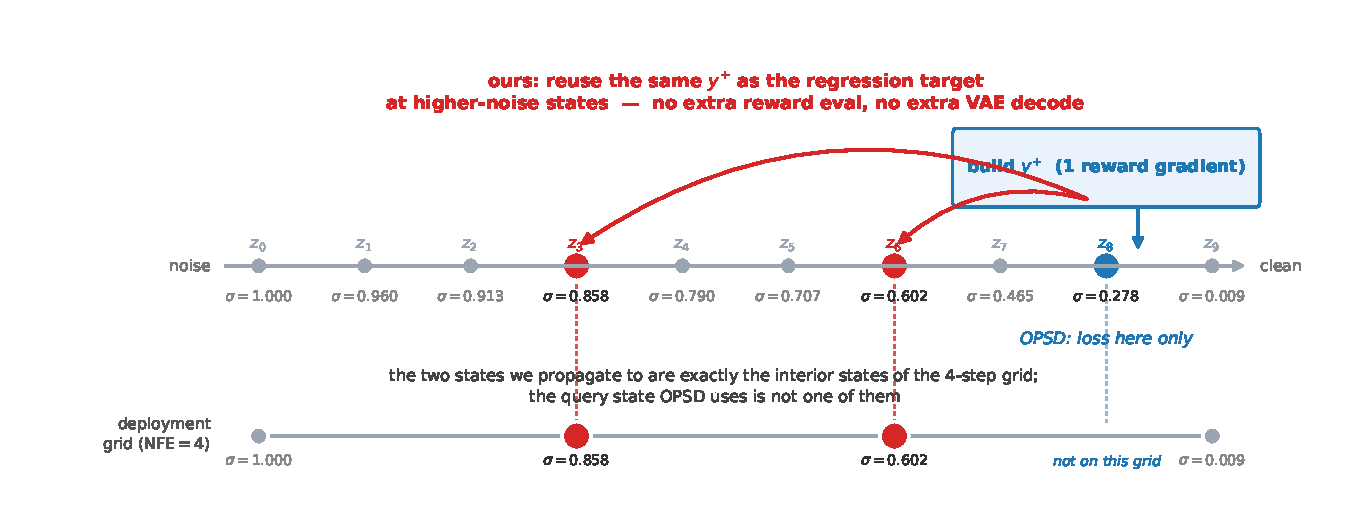
\includegraphics[width=\linewidth]{fig1_method.pdf}
\caption{\textbf{Where the reward target is applied.} The behavior policy produces a
rollout with schedule $\{\sigma_j\}$ (values shown are the actual SD3.5-M $10$-step
schedule). \opsd builds the detached target $\bar y_\pm$ at $z_8$ ($\sigma\!=\!0.278$) with
one reward gradient and applies its loss only there. \MSP reuses the \emph{same} target as
the regression target at $z_3$ and $z_6$ ($\sigma\!=\!0.858,\,0.602$), which requires no
further reward evaluation and no further decoding. The lower axis shows why those two
states: they are exactly the interior states of the four-step sampling grid
$\{1.000,\,0.858,\,0.602,\,0.009\}$, the grid the deployed model actually walks. \opsd's
query state is not on that grid at all, which is the sense in which its placement is tuned
for a different budget than the one a few-step deployment uses.}
\label{fig:method}
\end{figure}

\subsection{The target is type-correct at every noise level}

Equation~\eqref{eq:clean} defines a clean-output prediction \emph{for every query with
$\sigma>0$}, not only for the query at which the target was constructed. The detached
targets $\bar y_\pm$ of Eq.~\eqref{eq:targets} are points in that same clean-output space:
they are an estimate of a clean image, obtained by moving $y_0$ a bounded distance along
the reward gradient. Consequently, for any other state $z_k$ of the same rollout,
\begin{equation}
y_\theta(s_k)=z_k-\sigma_k v_\theta(s_k),\qquad s_k=(\vc,z_k,\sigma_k),
\end{equation}
is a quantity of the same type as $\bar y_\pm$, and regressing it onto $\bar y_\pm$ is
well-posed. This is the entire observation behind \MSP: \emph{a target built once can be
supervised many times}.

Two remarks delimit the claim. First, $\bar y_\pm$ is a target for the \emph{conditional
mean} at each state, not a claim that a single sample is reachable from $z_k$; this is
exactly the regression semantics that diffusion training already uses. Second, the
construction remains on-policy: all $z_k$ come from the same frozen-behavior-policy
trajectory that produced $z_q$.

\subsection{Objective}

Let $\mathcal K\subset\{1,\dots,N-1\}$, $q\notin\mathcal K$, be a set of additional states
of the same trajectory. \MSP replaces Eq.~\eqref{eq:opsdloss} by the uniform average
\begin{equation}
\boxed{\;
\mathcal L_{\MSP}
=\frac{1}{1+|\mathcal K|}
\Big[\;\mathcal L_{\mathrm{OPSD}}(s_q;\bar y_+,\bar y_-)
\;+\!\!\sum_{k\in\mathcal K}\!\mathcal L_{\mathrm{OPSD}}(s_k;\bar y_+,\bar y_-)\Big] \; }
\label{eq:msploss}
\end{equation}
where every term uses the \emph{same} $\bar y_\pm$, the same group weight $\omega$, and
its own adaptive normalizers $\gamma_\pm^{(k)}$ and branch anchor
$y_0^{(k)}=z_k-\sigma_k v_{\mathrm{old}}(s_k)$. The $1/(1+|\mathcal K|)$ factor keeps the
overall gradient scale comparable to the baseline; Sec.~\ref{sec:analysis} shows that this
down-weighting of the main term is not what drives the effect.

Throughout, our default is $\mathcal K=\{3,6\}$, i.e.\ $\sigma=0.858$ and $0.602$. These
are not tuned values. They are the two interior states of the $4$-step sampling grid
$\sigma\in\{1.000,\,0.858,\,0.602,\,0.009\}$ expressed on the $10$-step training grid
(all schedules are read from the model's own scheduler and listed in
App.~\ref{app:schedule}), and
we picked them for that reason; note that the canonical query $\sigma^\star\!=\!0.278$ lies
on neither grid, so \opsd supervises a state a $4$-step sampler never visits. What the data supports is
an \emph{interior optimum} in the noise level the set reaches. Replacing $\{3,6\}$ by the
lower, denser $\{5,6,7\}$ ($\sigma$ up to $0.707$) costs $2$--$3.5$ MDE at every budget from
$4$ to $40$ steps despite using \emph{more} states; replacing it by the \emph{higher}
$\{2,3,4\}$ ($\sigma$ up to $0.913$) is no better and is worse at the full budget
(App.~\ref{app:family}). The default sits between them. This matches the measured
reward-per-displacement exchange rate, which collapses from $0.457$ at $\sigma=0.278$ to
$0.007$ at $\sigma=0.913$ (Sec.~\ref{sec:analysis}): too little noise and the supervision
misses the states a few-step sampler visits, too much and the reward gradient has almost
no leverage there. Grid alignment alone does not explain the effect: among the budgets whose sampling grid has
an interior state at all, the advantage of $\{3,6\}$ over the lower set is \emph{smallest}
at exactly the budget it matches ($+2.2$ MDE at four steps, rising to $+3.5$ at twenty). At
two steps the grid has no interior state, and there the lower set is ahead by $4.8$ MDE
(App.~\ref{app:family}).

\subsection{Per-state backward is exact and memory-neutral}

Equation~\eqref{eq:msploss} is a sum of terms that share no intermediate activations:
each $\mathcal L_{\mathrm{OPSD}}(s_k;\cdot)$ requires its own forward pass of $v_\theta$
at $z_k$. Materializing all $1+|\mathcal K|$ graphs before a single backward would multiply
peak activation memory, which is prohibitive (the baseline already occupies
$79.2$ of $79.25$\,GiB on an A100). Because $\nabla_\theta$ is linear over the sum, we may
instead call backward once per state and let the gradients accumulate in
\texttt{.grad}:
\begin{equation}
\nabla_\theta\mathcal L_{\MSP}
=\frac{1}{1+|\mathcal K|}\Big[\nabla_\theta\mathcal L_{\mathrm{OPSD}}(s_q)
+\sum_{k\in\mathcal K}\nabla_\theta\mathcal L_{\mathrm{OPSD}}(s_k)\Big],
\end{equation}
which is \emph{exactly} the joint gradient while holding peak memory at the single-state
level. This is what makes the method practical rather than merely definable.

\subsection{Cost}

Each additional state costs two transformer forwards (behavior and trainable policy) and
one backward. It costs \emph{no} reward-model evaluation and \emph{no} VAE decode -- the
two dominant terms of target construction, which are incurred once regardless of
$|\mathcal K|$. Measured end-to-end over a full $100$-update run on identical hardware
(App.~\ref{app:cost}), $|\mathcal K|=2$ costs $1.21\times$ the baseline and
$|\mathcal K|=3$ costs $1.28\times$, i.e.\ $\approx\!+0.09$ to $+0.10\times$ per state.
